\documentclass{article}
\usepackage[utf8]{inputenc}

\title{Flowchart}
\author{praveen1460 }
\date{June 2015}

\usepackage{natbib}
\usepackage{graphicx}
\usepackage{tikz}
\usetikzlibrary{shapes.geometric, arrows}
\tikzstyle{startstop} = [rectangle, rounded corners, minimum width=1.5cm, minimum height=0.5cm,text centered, draw=black, fill=red!30]
\tikzstyle{io} = [trapezium, trapezium left angle=70, trapezium right angle=110, minimum width=1.5cm, minimum height=0.5cm, text centered, draw=black, fill=blue!30]
\tikzstyle{process} = [rectangle, minimum width=1.5cm, minimum height=0.5cm, text centered, text width=3cm, draw=black, fill=orange!30]
%\tikzstyle{decision} = [diamond, draw, minimum width=1.5cm, minimum height=0.5cm, text badly centered, draw=black, fill=green!30]
\tikzstyle{decision} = [diamond, draw, fill=green!30, 
    text width=5.6em, text badly centered, node distance=2cm, inner sep=0pt]
\tikzstyle{arrow} = [thick,->,>=stealth]

\begin{document}

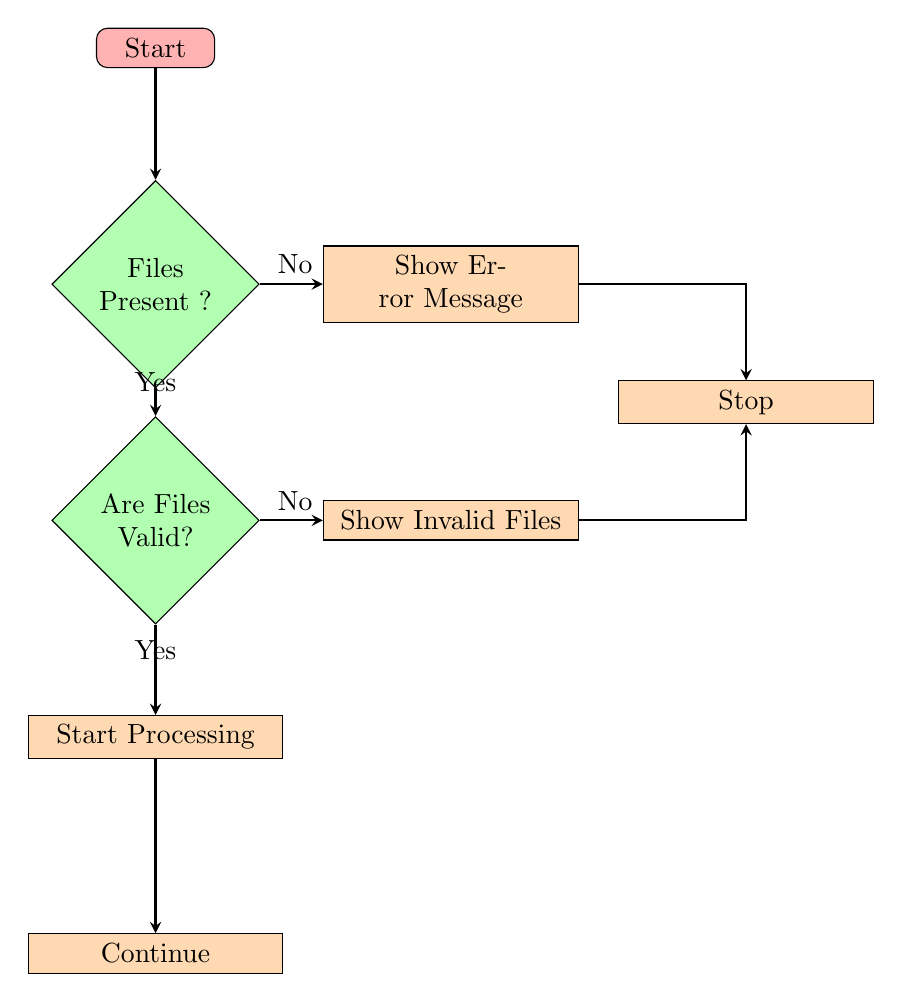
\begin{tikzpicture}[node distance=1.75 cm]

%% I/O, process, decision boxes

\node (start) [startstop] {Start};
\node (dec1)	[decision, below of=start, yshift = -1.0 cm]	{Files Present ?};
\node (dec2)	[decision, below of=dec1, yshift = -1.0 cm ]	{Are Files Valid?};
\node (pro1)	[process,  below of=dec2, yshift = -1.0 cm ]	{Start Processing};
\node (prod1)	[process,  right of=dec1, xshift = 2.0 cm ]	{Show Error Message};
\node (prod2)	[process,  right of=dec2, xshift = 2.0 cm ]	{Show Invalid Files};
\node (proEND)	[process,  right of=prod2, xshift= 2.0 cm, yshift = 1.5 cm] {Stop};
\node (pro2)	[process,  below of=pro1, yshift = -1.0 cm] {Continue};


%% Draw the connectivity.
\draw 	[arrow] (start)--(dec1);
\draw 	[arrow] (dec1)--node[anchor=south]{Yes}(dec2);
\draw 	[arrow] (dec2)--node[anchor=south]{Yes}(pro1);
\draw 	[arrow] (pro1)--(pro2);
\draw 	[arrow] (dec1)--node[anchor=east, yshift=0.25cm, xshift=0.4cm]{No}(prod1);
\draw 	[arrow] (dec2)--node[anchor=east, yshift=0.25cm, xshift=0.4cm]{No}(prod2);
\draw 	[arrow] (prod2)-|(proEND);
\draw 	[arrow]	(prod1)-|(proEND);
\end{tikzpicture}




\end{document}

